\documentclass[letterpaper,9pt,twocolumn,twoside,]{pinp}

%% Some pieces required from the pandoc template
\providecommand{\tightlist}{%
  \setlength{\itemsep}{0pt}\setlength{\parskip}{0pt}}

% Use the lineno option to display guide line numbers if required.
% Note that the use of elements such as single-column equations
% may affect the guide line number alignment.

\usepackage[T1]{fontenc}
\usepackage[utf8]{inputenc}

% pinp change: the geometry package layout settings need to be set here, not in pinp.cls
\geometry{layoutsize={0.95588\paperwidth,0.98864\paperheight},%
  layouthoffset=0.02206\paperwidth, layoutvoffset=0.00568\paperheight}

\definecolor{pinpblue}{HTML}{185FAF}  % imagecolorpicker on blue for new R logo
\definecolor{pnasbluetext}{RGB}{101,0,0} %



\title{Predicting Concrete Compressive Strength using Multiple Linear
Regression}

\author[]{Jonathan Then}
\author[]{Lihai Geng}
\author[]{Yan Liu}
\author[]{Yujia Zhai}

  \affil[]{University of Sydney, Camperdown, New South Wales, Sydney, Australia,
2006}

\setcounter{secnumdepth}{0}

% Please give the surname of the lead author for the running footer
\leadauthor{}

% Keywords are not mandatory, but authors are strongly encouraged to provide them. If provided, please include two to five keywords, separated by the pipe symbol, e.g:
 

\begin{abstract}
This report demonstrates the process of using Multiple Linear Regression
on predicting concrete compressive strength of 28 days using the
Concrete dataset. The data exploration is performed to visualise initial
observations between all predictors and the target. Detailed analysis on
the model selection process are presented to give the final chosen
model. Further inference, interpretion and performance analysis on final
model led to the conclusion of this process.
\end{abstract}

\dates{This version was compiled on \today} 


% initially we use doi so keep for backwards compatibility
% new name is doi_footer
\doifooter{\url{https://cran.r-project.org/package=pinp}}

\pinpfootercontents{T11A\_Ontime\_6}

\begin{document}

% Optional adjustment to line up main text (after abstract) of first page with line numbers, when using both lineno and twocolumn options.
% You should only change this length when you've finalised the article contents.
\verticaladjustment{-2pt}

\maketitle
\thispagestyle{firststyle}
\ifthenelse{\boolean{shortarticle}}{\ifthenelse{\boolean{singlecolumn}}{\abscontentformatted}{\abscontent}}{}

% If your first paragraph (i.e. with the \dropcap) contains a list environment (quote, quotation, theorem, definition, enumerate, itemize...), the line after the list may have some extra indentation. If this is the case, add \parshape=0 to the end of the list environment.


\hypertarget{introduction}{%
\subsection{Introduction}\label{introduction}}

The main aim of this report is to demonstrate the possibilities of
adapting Multiple Linear Regression (MLR) to predict the concrete
compressive strength of 28 days using the Concrete dataset.The main
question to answer is: Are all variables in the dataset significantly in
predicting the concrete compressive strength of 28 days?

\hypertarget{dataset}{%
\subsection{Dataset}\label{dataset}}

The dataset can be found on the UCI machine learning repository. Here is
the link :
\url{https://archive.ics.uci.edu/ml/datasets/Concrete+Compressive+Strength}.
It is donated by its original owner --- Professor I-Cheng Yeh,
Department of Information Management Chung-Hua University, Hsin Chu,
Taiwan 30067, R.O.C..In the original paper, experimental data came from
17 different sources. So during the data collection, there is a
determination made to ensure that all these mixtures are fairly
representative group governing all of the major parameters that
influence the strength of high-performance concrete, for example, they
deleted some observations which contain larger aggregates. In this
dataset, there are 1030 observations with 9 quantitative variables There
is one dependent variable Compressive Concrete Strength, which is the
index used to show how much pressure the concrete can withstand.
Opposite with that one, the other 8 variables are all independent
variables. They are

\begin{itemize}
\tightlist
\item
  Cement, a kind of binder, is used for combining materials together.
\item
  Blast Furnace Slag, is a non-metallic coproduct in the production of
  iron.
\item
  Fly Ash, which can improve the strength and segregation of the
  concrete and make concrete easier to pump.
\item
  Water, used to form a paste that binds the aggregates together.
\item
  Superplasticizers, they are chemical compounds using for reducing
  water in the production of concrete.
\item
  Coarse Aggregate \& Fine Aggregate, they are particles free of
  absorbed chemicals or coatings of clay and other fine materials that
  could cause the deterioration of concrete.
\item
  Age, the number of days that how long has the concrete been made for
  And there are no missing values in this dataset.
\end{itemize}

\hypertarget{analysis}{%
\subsection{Analysis}\label{analysis}}

The dataset was cleaned and filtered to only include data points where
the concrete was tested at 28 days in order to answer our main question.
The resulting dataset contains 425 observations.

\hypertarget{data-exploration}{%
\subsubsection{Data Exploration}\label{data-exploration}}

Initial data exploration was conducted to see if there was any linear
relationship between our dependent variable, strength, when compared to
all the other variables. By looking at the correlation coefficient and
the ggpairs plot, we can infer that cement has a strong positive linear
relationship, water has a negative linear relationship, while the rest
has a weak relationship with strength. From there, we decided to use a
full model containing all predictors in the dataset so as to find out
the p-values when fitted on a multiple linear regression.

\begin{ShadedResult}
\begin{verbatim}
#              Estimates p-value
#  Intercept   -95.67    0.17   
#  Cement      0.14      0.11   
#  Slag        -0.06     0.11   
#  FlyAsh      0.04      0.05   
#  Water       0.001     <0.001 
#  Plasticizer <0.001    <0.001 
#  Coarse Agg  0.126     0.260  
#  Fine Agg    <0.001    <0.001
\end{verbatim}
\end{ShadedResult}

\begin{itemize}
\tightlist
\item
  Both the p-values of water and plasticizer are greater than 0.05.
  Therefore, they are insignificant at the 5\% level of significance.
\item
  We cannot immediately drop both of them from the model as the p-values
  are only testing individual coefficients.
\item
  The AIC for the full model is 2881.297.
\end{itemize}

\hypertarget{backward-forward-selection-model}{%
\subsubsection{Backward \& Forward Selection
Model}\label{backward-forward-selection-model}}

Stepwise model selection methods of forward and backward selection were
used to select the final model.

\begin{ShadedResult}
\begin{verbatim}
#             Estimates p-value Estimates p-value
#  Intercept  -81.93    0.003   -81.93    0.003  
#  Cement     0.17      <0.001  0.17      <0.001 
#  Slag       0.14      <0.001  0.14      <0.001 
#  FlyAsh     0.11      <0.001  0.11      <0.001 
#  Water      -0.09     0.012   -0.09     0.012  
#  Coarse Agg 0.04      <0.001  0.04      <0.001 
#  Fine Agg   0.05      <0.001  0.05      <0.001
\end{verbatim}
\end{ShadedResult}

\begin{ShadedResult}
\begin{verbatim}
#                   Backward Model Forward Model
#  Observations     425            425          
#  R^2/R^2 Adjusted 0.771/0.767    0.771/0.767  
#  AIC              2880.591       2880.591
\end{verbatim}
\end{ShadedResult}

Both forward and backward models arrived at the same model and has
slightly lower AIC when compared to the full model. Therefore, this will
be our final model.

\hypertarget{assumptions-checking-refer-to-figure-1}{%
\subsubsection{Assumptions Checking (Refer to Figure
1)}\label{assumptions-checking-refer-to-figure-1}}

\begin{itemize}
\tightlist
\item
  Linearity: There is a slight curved pattern in the residual vs fitted
  values plot. We are overestimating concrete strength for low and high
  fitted values.
\item
  Independence: It is assumed that the observations are not related to
  one another as this was dealt with in the experimental design phase,
  before data collection.
\item
  Homoscedasticity: There does seem to be some fanning out of the
  residuals in the residual vs fitted value plot, indicating that there
  may be some heteroscedasticity in our data.
\item
  Normality: Based on the QQPlot, the bottom and top points are not on
  the line. However, we could appeal to the Central Limit Theorem
  because we have a reasonable amount of observations meaning our
  inferences are approximately valid.
\end{itemize}

\hypertarget{results}{%
\subsection{Results}\label{results}}

The final model is

Strength = -81.93 + 0.17(Cement) + 0.14(Blast Furnace Slag) + 0.11(Fly
Ash) - 0.09(Water) + 0.05(Fine Aggregate) + 0.04(Coarse Aggregate) +
\(\epsilon\)

\hypertarget{interpretation}{%
\subsubsection{Interpretation}\label{interpretation}}

Holding all other variables constant:

\begin{itemize}
\tightlist
\item
  Increase in 1 \(kg/m^3\) of Cement results in 0.17 \(MPa\) increase in
  strength on average.
\item
  Increase in 1 \(kg/m^3\) of Blast Furnace Slag results in 0.14 \(MPa\)
  increase in strength on average.
\item
  Increase in 1 \(kg/m^3\) of Fly Ash results in 0.11 \(MPa\) increase
  in strength on average.
\item
  Increase in 1 \(kg/m^3\) of Water results in 0.09 \(MPa\) decrease in
  strength on average.
\item
  Increase in 1 \(kg/m^3\) of Fine Aggregate results in 0.05 \(MPa\)
  increase in strength of on average.
\item
  Increase in 1 \(kg/m^3\) of Coarse Aggregate results in 0.11 \(MPa\)
  increase in strength on average.
\end{itemize}

\hypertarget{statistical-inference}{%
\subsubsection{Statistical Inference}\label{statistical-inference}}

Individual t -- test was conducted on each slope parameter to check if
it is significantly different from zero, i.e significantly in predicting
strength. The test procedures are as follows:

\textbf{Hypothesis:} \(H_{0}: \beta_{i} = 0\) vs
\(H_{1}:\beta_{i} \neq 0\)

\textbf{Assumptions:} The residuals are iid normal distribution with
mean of zero and constant variance of \({\sigma}^2\) and there is a
linear relationship between strength and each predictor.

\textbf{P-value:} Each of the p-value is less than 0.05.

\textbf{Decision:} We reject the null hypothesis and conclude that there
is very strong evidence in the data to indicate a linear relationship
between each predictor and the strength.

However, since there is a slight heteroscedasticity in our data, the
inference might be invalid.

\hypertarget{performance}{%
\subsubsection{Performance}\label{performance}}

\begin{ShadedResult}
\begin{verbatim}
#                     Full Model Final Model
#  Adjusted R Squared     0.7733      0.7699
#  RMSE                   7.1688      7.0898
#  MAE                    5.3890      5.3254
\end{verbatim}
\end{ShadedResult}

10-folds cross validation method was used to fit the full model and the
final model to compare performance results.

\begin{itemize}
\tightlist
\item
  In Sample Performance: The full model has a slightly higher adjusted
  \(R^2\), indicating a stronger fit of the model as compared to the
  final model. The adjusted \(R^2\) indicates how much percentage of
  total variability in strength is explained by the model.
\item
  Out of Sample Performance: The Root Mean Squared Error (RMSE) is the
  square root of the variance of the residuals and the Mean Absolute
  Error (MAE) is the average over the absolute differences between
  prediction and actual observation. A smaller RMSE and MAE is desired.
  The final model has a lower RMSE and MAE, indicating that it is better
  at predicting observations that are not used to build the model. This
  is another reason why the final model was chosen.
\end{itemize}

\hypertarget{discussion-and-conclusion}{%
\subsection{Discussion and Conclusion}\label{discussion-and-conclusion}}

\hypertarget{conclusion}{%
\subsubsection{Conclusion}\label{conclusion}}

Based on the final model, Super Plasticizer is excluded in the multiple
linear regression model because it is not significant for predicting
concrete compressive strength of 28 days.

\hypertarget{limitation}{%
\subsubsection{Limitation}\label{limitation}}

According to the assumption checking of the final model, there is slight
heteroscedasticity in the data, so the standard errors computed for the
least squares estimators are incorrect. This can affect confidence
intervals and hypothesis testing that use those standard errors, which
could lead to misleading conclusions.

\hypertarget{improvement}{%
\subsubsection{Improvement}\label{improvement}}

This limitation can be improved by using robust standard errors to
correct the issue of incorrect standard errors so that the interval
estimates and hypothesis tests are valid.

\hypertarget{references}{%
\subsection{References}\label{references}}

\begin{itemize}
\tightlist
\item
  Gopal Mishra. (2014, October). Factors Affecting Strength of Concrete.
  The Constructor.
  \url{https://theconstructor.org/concrete/factors-affecting-strength-of-concrete/6220/Humad},
  A. M. (2019).
\item
  \url{https://www.frontiersin.org/articles/10.3389/fmats.2019.00009/fullPatel},
  H. (2019, November 9). 11 Factors that can Affect the Strength of
  Concrete. GharPedia.
\item
  \url{https://gharpedia.com/blog/factors-that-affect-strength-of-concrete/Portland}
  Cement Association. (n.d.). Aggregates. Retrieved November 10, 2020,
  from
\item
  Association. (n.d.). Slag Cement Questions. Retrieved November 10,
  2020, from
  \url{https://www.slagcement.org/resources/faqs.aspxStelsel}, K. (2015,
  March 7). Using Fly Ash in Concrete. National
\item
  Yeh, I.C. (1998). Modeling of strength of high-performance concrete
  using artificial neural networks. Cement and Concrete Research, Vol.
  28, No.~12, pp.~1797--1808, DOI:~10.1016/S0008-8846(98)00165-3
\item
  `Cement'. (n.d.). ~In Wikipedia. Retrieved November 13, 2020, from
  \url{https://en.wikipedia.org/wiki/Cement}
\item
  U.S. Department of transportation Federal Highway Administration.
  (2016). User Guidelines for Waste and Byproduct Materials in Pavement
  Construction. Retrieved from
  \url{https://www.fhwa.dot.gov/publications/research/infrastructure/structures/97148/bfs1.cfm}
\item
  Rodriguez, J. (2019). Uses, Benefits, and Drawbacks of Fly Ash in
  Construction. Retrieved from
  \url{https://www.thebalancesmb.com/fly-ash-applications-844761}
\item
  `Superplasticizer'. (n.d.). ~In Wikipedia. Retrieved November 13,
  2020, from \url{https://en.wikipedia.org/wiki/Superplasticizer}
\item
  Aggregates. (2019). Portland Cement Association. Retrieved from
  \url{https://www.cement.org/cement-concrete-applications/concrete-materials/aggregates}
\end{itemize}

\hypertarget{link-to-github}{%
\subsection{Link to GitHub}\label{link-to-github}}

\begin{itemize}
\tightlist
\item
  \url{https://github.sydney.edu.au/YZHA2588/T11A_Ontime_6}
\end{itemize}

\begin{figure*}
  \begin{center}
    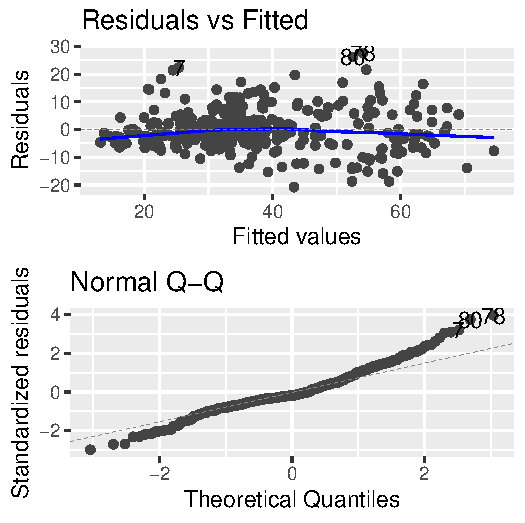
\includegraphics[width=0.66\textwidth, height=5in]{resid} 
  \end{center}
  \caption{Residuals vs Fitted Plots and QQPlot}\label{fig}
\end{figure*}

%\showmatmethods


\bibliography{pinp}
\bibliographystyle{jss}



\end{document}

